\documentclass[aspectratio=169]{beamer}

\graphicspath{{figs}}

\usepackage{iftex}
\ifPDFTeX
    \usepackage[T2A]{fontenc}
    \usepackage[utf8]{inputenc}
\else
    \usepackage{fontspec}
    \setmainfont{cmunrm.otf}[BoldFont=cmunbx.otf,ItalicFont=cmunti.otf]
    \setsansfont{cmunss.otf}[BoldFont=cmunsx.otf,ItalicFont=cmunsi.otf]
\fi
\usepackage[english,russian]{babel}
\usepackage{cmap}
\usepackage{tikz}
\usepackage{array}
\usepackage{multirow}
\usepackage{multicol}
\usepackage{booktabs}
\usepackage{csquotes}
\usepackage{amssymb,amsfonts,amsmath}

\usecolortheme{beaver}
\usefonttheme[onlymath]{serif}
\setbeamertemplate{navigation symbols}{}
\setbeamertemplate{footline}[page number]
\setbeamertemplate{blocks}[rounded=true,shadow=false]
\setbeamertemplate{itemize items}[circle]
\setbeamersize{text margin left=0.6cm,text margin right=0.6cm}
\setbeamertemplate{frametitle}[default][center]
\setbeamercolor{frametitle}{fg=black}

\definecolor{accent}{HTML}{8B1A1A}
\definecolor{soft}{HTML}{6B6B6B}
\setbeamercolor{block title}{bg=blue!10, fg=blue!50!black}
\setbeamercolor{block body}{bg=blue!3}
\setbeamercolor{block title alerted}{bg=accent!12, fg=accent}
\setbeamercolor{block body alerted}{bg=accent!3}
\setbeamercolor{block title example}{bg=green!12, fg=green!35!black}
\setbeamercolor{block body example}{bg=green!3}

\newcommand{\Rk}[1]{\mathrm{Recall@}#1}
\newcommand{\src}[1]{{\scriptsize\color{soft} #1}}

\begin{document}

%%%%%%%%%%%%%%%%%%%%%%%%%%%%%%%%%%%%%%%%%%%%%%%%%%%%%%%%%%%%
\begin{frame}[plain,t]
    \centering
    \vspace*{1.0cm}
    {\usebeamercolor[fg]{title}\LARGE\bfseries Сравнение стратегий разбиения\\[3pt] патентных документов\\[3pt] для семантического поиска и RAG\par}

    \vspace{0.5cm}
    \begin{tikzpicture}\draw[accent, line width=1.2pt] (0,0) -- (6,0);\end{tikzpicture}

    \vspace{0.7cm}
    {\Large Елизавета Кожемякова\par}

    \vspace{0.5cm}
    {\color{soft}\normalsize Научный руководитель\par}
    \vspace{2pt}
    {\large Роман Ищенко\par}

    \vspace{0.9cm}
    {\color{soft}\small 2026\par}
\end{frame}

%%%%%%%%%%%%%%%%%%%%%%%%%%%%%%%%%%%%%%%%%%%%%%%%%%%%%%%%%%%%
\begin{frame}{Зачем разбивать патент по разделам}
    \small
    \begin{columns}[T]
        \begin{column}{0.48\textwidth}
            \begin{alertblock}{Проблема}
                Поиск и RAG видят патент только через найденные фрагменты.
                Разбиение по длине смешивает в одном фрагменте разные разделы, например конец уровня техники и начало сущности изобретения.
                Неясно, как это влияет на поиск.
            \end{alertblock}
            \begin{block}{Цель}
                Найти схему разбиения патентов, которая повышает качество поиска при той же модели векторов, без LLM при индексации и без обучения.
            \end{block}
        \end{column}
        \begin{column}{0.48\textwidth}
            \begin{block}{Гипотеза}
                Фрагменты, не пересекающие границы разделов, ищутся точнее, чем фрагменты фиксированной длины.
            \end{block}
            \begin{exampleblock}{Что сделано}
                \begin{enumerate}[1)]
                    \item Разделы найдены автоматически у 98,5\% из 37\,727 патентов.
                    \item Разбиение по разделам сравнено с разбиением по длине при трех способах поиска и двух видах запросов.
                    \item Найдено, где теряется качество.
                \end{enumerate}
            \end{exampleblock}
        \end{column}
    \end{columns}
\end{frame}

%%%%%%%%%%%%%%%%%%%%%%%%%%%%%%%%%%%%%%%%%%%%%%%%%%%%%%%%%%%%
\begin{frame}[t]{Фрагменты не пересекают разделы}
    \begin{alertblock}{Суть}
        \footnotesize
        Разбиение по длине смешивает в одном фрагменте разные разделы патента.
        Строим фрагменты $c_j$ по разделам $s_k$, чтобы смысл не размывался, а вклад каждого раздела в поиск можно было измерить.
    \end{alertblock}

    \begin{columns}[T]
        \begin{column}{0.55\textwidth}
            \begin{block}{Термины и обозначения}
                \footnotesize
                \textbf{Патент} $d$: документ из разделов $s_k$.\\
                \textbf{Разбиение} $\varphi$: деление $d$ на фрагменты $c_j$.\\
                \textbf{Векторный поиск}: выбор $c_j$, близких к запросу по эмбеддингам.\\
                \textbf{RAG}: ответ языковой модели по найденным $c_j$.
            \end{block}
            \vspace{-4pt}
            \centering
            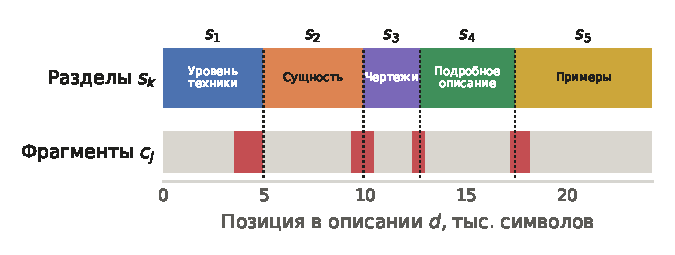
\includegraphics[width=0.72\textwidth]{sections_chunks}
        \end{column}
        \begin{column}{0.43\textwidth}
            \begin{exampleblock}{Результат}
                \footnotesize
                \begin{itemize}
                    \item 10,1\% фрагментов по длине пересекают границу раздела (красные на рисунке).
                    \item После переранжирования разбиение по разделам поднимает $\Rk{1}$ на 0,05--0,07 во всех схемах без расширения запросов.
                    \item Способ поиска важнее разбиения: BM25 точнее векторного поиска на 0,08--0,10 по $\Rk{1}$.
                \end{itemize}
            \end{exampleblock}
        \end{column}
    \end{columns}
\end{frame}

%%%%%%%%%%%%%%%%%%%%%%%%%%%%%%%%%%%%%%%%%%%%%%%%%%%%%%%%%%%%
\begin{frame}{Что уже предложено}
    \footnotesize
    \centering
    \renewcommand{\arraystretch}{1.1}
    \begin{tabular}{>{\raggedright\arraybackslash}p{0.27\textwidth}>{\raggedright\arraybackslash}p{0.3\textwidth}>{\raggedright\arraybackslash}p{0.34\textwidth}}
        \toprule
        \textbf{Метод} & \textbf{Сильные стороны} & \textbf{Слабые стороны} \\
        \midrule
        Длина, группы абзацев\newline \src{Shaukat и др., 2026} & Просто, группы абзацев лучшие из дешевых & Режут посреди мысли, в патентах почти нет разметки абзацев \\
        По заголовкам\newline \src{Taiwo, Yusoff, 2026} & MRR 0,64 против 0,59, индекс в 4 раза меньше & Заголовки из разметки, не патенты, без переранжирования \\
        RAPTOR\newline \src{Sarthi и др., 2024} & Поиск на нескольких уровнях & Много вызовов LLM при индексации \\
        DAPFAM\newline \src{Ayaou и др., 2025} & Поиск по фрагментам патента лучше, чем по целому & Только окна фиксированной длины, разделы не учитываются \\
        BM25\newline \src{Robertson, Zaragoza, 2009} & Точно совпадает по редким терминам, без обучения и GPU & Не видит синонимов и перефразировок \\
        PAI-NET, PaECTER\newline \src{Lee, Bai, 2025. Ghosh и др., 2024} & Учитывают специфику патентов & Требуют обучения модели \\
        \midrule
        \textbf{По разделам} (наша) & Роль разделов патента, готовая модель, без LLM & Правила поиска заголовков зависят от типа документов \\
        \bottomrule
    \end{tabular}

    \medskip
    \raggedright
    Разбиение по заголовкам проверено на корпоративных документах, но не на патентах и не с переранжированием.
\end{frame}

%%%%%%%%%%%%%%%%%%%%%%%%%%%%%%%%%%%%%%%%%%%%%%%%%%%%%%%%%%%%
\begin{frame}{Постановка задачи}
    \footnotesize
    \begin{columns}[T]
        \begin{column}{0.48\textwidth}
            \begin{block}{Дано}
                Корпус $D=\{d_1,\dots,d_N\}$, $N = 37\,727$. Патент $d$ состоит из реферата, описания с разделами $s_1,\dots,s_K$ и формулы.\\[3pt]
                Вопросы $Q = \{(q_i, p_i, E_i)\}_{i=1}^{150}$, где $p_i$ нужный патент, $E_i$ доказательства из его текста.
            \end{block}
            \begin{block}{Модель поиска (фиксирована)}
                Разбиение $\varphi: d \mapsto \{c_j\}$. Оценка $\sigma(q, c)$: косинус эмбеддингов, BM25 или их RRF.
                Топ-50 фрагментов по $\sigma$ переупорядочивает кросс-энкодер $r(q, c)$.
            \end{block}
        \end{column}
        \begin{column}{0.48\textwidth}
            \begin{block}{Критерии качества}
                $\pi_i(\varphi)$: место $p_i$ среди патентов выдачи.
                \[
                    \Rk{k}(\varphi) = \frac{1}{|Q|}\sum_{i=1}^{|Q|} \bigl[\pi_i(\varphi) \le k\bigr]
                \]
                MRR: среднее $1/\pi_i(\varphi)$.
                $\mathrm{EvHit@}k$: доля вопросов, где фрагмент с доказательством попал в первые $k$ фрагментов.
            \end{block}
            \begin{alertblock}{Задача}
                \[
                    \varphi^* = \arg\max_{\varphi \in \Phi} \Rk{k}(\varphi)
                \]
                $\Phi = \{\varphi_{\text{длина}}, \varphi_{\text{разделы}}\}$, $\sigma$ и $r$ фиксированы.
            \end{alertblock}
        \end{column}
    \end{columns}
\end{frame}

%%%%%%%%%%%%%%%%%%%%%%%%%%%%%%%%%%%%%%%%%%%%%%%%%%%%%%%%%%%%
\begin{frame}{Разбиение по разделам}
    \footnotesize
    \begin{columns}[T]
        \begin{column}{0.52\textwidth}
            \begin{block}{Алгоритм $\varphi_{\text{разделы}}$}
                \textbf{Вход:} патент $d$, окно $n=10$ предложений, перекрытие $o=1$, словарь заголовков.
                \begin{enumerate}[1)]
                    \item Реферат и формулу считать отдельными частями.
                    \item В описании найти заголовки из словаря. Они задают границы разделов $s_k$.
                    \item Каждую часть делить окнами по $n$ предложений с перекрытием $o$, не выходя за ее границу.
                \end{enumerate}
                \textbf{Выход:} фрагменты $c_j$, каждый с типом своего раздела.
            \end{block}
            {\color{soft}Базовое разбиение $\varphi_{\text{длина}}$ делит склеенный текст патента теми же окнами.}
        \end{column}
        \begin{column}{0.44\textwidth}
            \begin{exampleblock}{Свойства}
                \begin{itemize}
                    \item Нет LLM и обучения, модель векторов та же.
                    \item Размер окна тот же, поэтому сравнение показывает эффект именно границ.
                    \item Индекс на 6,5\% больше: 47,9 фрагмента на патент против 45,0.
                    \item Уровень техники и сущность изобретения получают 1--2 собственных фрагмента.
                \end{itemize}
            \end{exampleblock}
        \end{column}
    \end{columns}
\end{frame}

%%%%%%%%%%%%%%%%%%%%%%%%%%%%%%%%%%%%%%%%%%%%%%%%%%%%%%%%%%%%
\begin{frame}{Данные}
    \footnotesize
    \begin{columns}[T]
        \begin{column}{0.32\textwidth}
            \begin{block}{Корпус патентов}
                37\,727 патентов США по покрытиям и обработке поверхностей.
                \medskip

                У каждого есть реферат, описание и формула.
                \medskip

                Разметки разделов и абзацев нет, заголовки записаны прописными буквами прямо в тексте.
            \end{block}
        \end{column}
        \begin{column}{0.32\textwidth}
            \begin{block}{Вопросы}
                150 вопросов по патентам корпуса.
                \medskip

                Для каждого известны нужный патент, ответ и фрагмент текста с доказательством.
                \medskip

                Ответ взят из реферата (74), формулы (61) или описания (15). 10 вопросов сравнивают два патента.
            \end{block}
        \end{column}
        \begin{column}{0.32\textwidth}
            \begin{block}{Расширенные вопросы}
                Те же 150 вопросов, переписанные языковой моделью в развернутый текст в стиле реферата.
                \medskip

                Медиана 140 слов против 15 у исходных.
                \medskip

                По ним идет поиск, а переранжирование по исходному вопросу.
            \end{block}
        \end{column}
    \end{columns}

    \bigskip
    \begin{alertblock}{Что проверяем}
        Как разбиение по разделам работает на всем корпусе, на исходных и на расширенных вопросах, при трех способах поиска.
    \end{alertblock}
\end{frame}

%%%%%%%%%%%%%%%%%%%%%%%%%%%%%%%%%%%%%%%%%%%%%%%%%%%%%%%%%%%%
\begin{frame}{Эксперимент 1. Поиск разделов}
    \footnotesize
    \begin{columns}[T]
        \begin{column}{0.48\textwidth}
            \begin{block}{Что обнаружено}
                В описаниях нет разметки, но заголовки разделов записаны прописными буквами прямо в тексте, например BACKGROUND OF THE INVENTION.
            \end{block}
            \begin{block}{Как ищем}
                \begin{enumerate}[1)]
                    \item Берем слова прописными буквами в начале предложений.
                    \item Оставляем варианты, встречающиеся хотя бы в 20 патентах.
                    \item По ключевым словам относим к одному из 8 типов: BACKGROUND к уровню техники, SUMMARY к сущности изобретения и т.\,д.
                \end{enumerate}
            \end{block}
        \end{column}
        \begin{column}{0.48\textwidth}
            \centering
            \setlength{\tabcolsep}{3pt}
            \begin{tabular}{lccc}
                \toprule
                \textbf{Раздел} & \textbf{Патентов} & \textbf{Текста} & \textbf{Предл.} \\
                \midrule
                Подробное описание & 89\% & 63\% & 180 \\
                Примеры & 46\% & 25\% & 78 \\
                Сущность изобретения & 86\% & 13\% & 18 \\
                Уровень техники & 91\% & 8\% & 16 \\
                Чертежи & 75\% & 6\% & 14 \\
                Связанные заявки & 56\% & 4\% & 7 \\
                Область техники & 58\% & 1\% & 2 \\
                \bottomrule
            \end{tabular}

            \medskip
            \begin{exampleblock}{Результат}
                \begin{itemize}
                    \item 291 вариант заголовка сведен к 8 типам.
                    \item Разделы найдены у 98,5\% патентов, в среднем 5,15 типа.
                    \item 10,1\% фрагментов по длине пересекают границу раздела.
                \end{itemize}
            \end{exampleblock}
        \end{column}
    \end{columns}
\end{frame}

%%%%%%%%%%%%%%%%%%%%%%%%%%%%%%%%%%%%%%%%%%%%%%%%%%%%%%%%%%%%
\begin{frame}{Эксперимент 2. Разбиение и качество поиска}
    \small
    \begin{block}{Как сравниваем}
        Строим два индекса корпуса, по длине и по разделам, и на каждом ищем нужный патент для всех 150 вопросов разными способами поиска.
    \end{block}
    \begin{columns}[T]
        \begin{column}{0.48\textwidth}
            \begin{block}{Меняется}
                \begin{tabular}{@{}ll@{}}
                    Разбиение & по длине, по разделам \\
                    Поиск & векторный, BM25, гибридный \\
                    Запросы & исходные, расширенные \\
                \end{tabular}
            \end{block}
        \end{column}
        \begin{column}{0.48\textwidth}
            \begin{block}{Фиксировано}
                Эмбеддер bge-small-en-v1.5, переранжировщик bge-reranker-base, 50 фрагментов в выдаче, окно 10 предложений.
            \end{block}
        \end{column}
    \end{columns}
    \begin{exampleblock}{Статистика}
        10 прогонов. 95\% бутстреп-интервалы и парные сравнения на тех же вопросах с поправкой Холма.
    \end{exampleblock}
\end{frame}

%%%%%%%%%%%%%%%%%%%%%%%%%%%%%%%%%%%%%%%%%%%%%%%%%%%%%%%%%%%%
\begin{frame}{Результаты всех прогонов}
    \footnotesize
    \centering
    \setlength{\tabcolsep}{4pt}
    \renewcommand{\arraystretch}{1.1}
    \begin{tabular}{llccccc}
        \toprule
        & & \textbf{До} & \multicolumn{4}{c}{\textbf{После переранжирования}} \\
        \cmidrule(lr){3-3}\cmidrule(lr){4-7}
        \textbf{Разбиение} & \textbf{Поиск} & $\Rk{1}$ & $\Rk{1}$ & $\Rk{10}$ & MRR & EvHit@5 \\
        \midrule
        \multirow{5}{*}{По длине} & Векторный & 0,52 & 0,55 & 0,83 & 0,66 & 0,63 \\
        & BM25 & \textbf{0,69} & 0,65 & 0,93 & 0,75 & 0,75 \\
        & Гибридный & 0,65 & 0,63 & 0,92 & 0,74 & 0,75 \\
        & Векторный + расширение & 0,49 & 0,55 & 0,78 & 0,64 & 0,61 \\
        & Гибридный + расширение & 0,37 & 0,60 & 0,77 & 0,67 & 0,62 \\
        \midrule
        \multirow{5}{*}{По разделам} & Векторный & 0,51 & 0,63 & 0,86 & 0,71 & 0,61 \\
        & BM25 & 0,68 & \textbf{0,71} & \textbf{0,93} & \textbf{0,79} & \textbf{0,77} \\
        & Гибридный & 0,65 & 0,70 & 0,92 & 0,78 & 0,75 \\
        & Векторный + расширение & 0,51 & 0,61 & 0,77 & 0,67 & 0,57 \\
        & Гибридный + расширение & 0,37 & 0,57 & 0,77 & 0,65 & 0,59 \\
        \bottomrule
    \end{tabular}

    \medskip
    \raggedright
    Лучший прогон: разбиение по разделам с BM25. Интервал для $\Rk{1}$ около $\pm$0,07.\\
    Расширение запросов не улучшило ни одну метрику ни в одной схеме.
\end{frame}

%%%%%%%%%%%%%%%%%%%%%%%%%%%%%%%%%%%%%%%%%%%%%%%%%%%%%%%%%%%%
\begin{frame}{Разделы помогают после переранжирования}
    \footnotesize
    {\color{soft}Для каждого способа поиска сравниваем $\Rk{1}$ на двух индексах до и после переранжирования.}

    \centering
    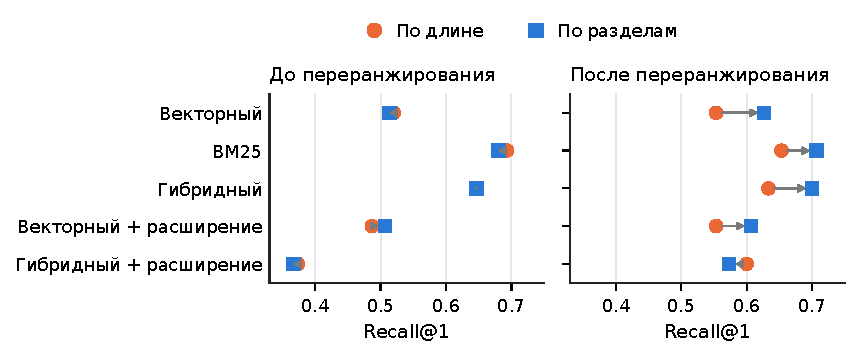
\includegraphics[width=0.84\textwidth]{mtalk_sections}

    \raggedright
    \begin{itemize}
        \item До переранжирования разбиения неразличимы: разность от $-$0,01 до +0,02.
        \item После него разбиение по разделам лучше во всех трех схемах без расширения, на 0,05--0,07.
        \item Кросс-энкодер точнее оценивает фрагмент, не смешивающий разделы.
    \end{itemize}
\end{frame}

%%%%%%%%%%%%%%%%%%%%%%%%%%%%%%%%%%%%%%%%%%%%%%%%%%%%%%%%%%%%
\begin{frame}{Что значимо}
    \begin{columns}[c]
        \begin{column}{0.6\textwidth}
            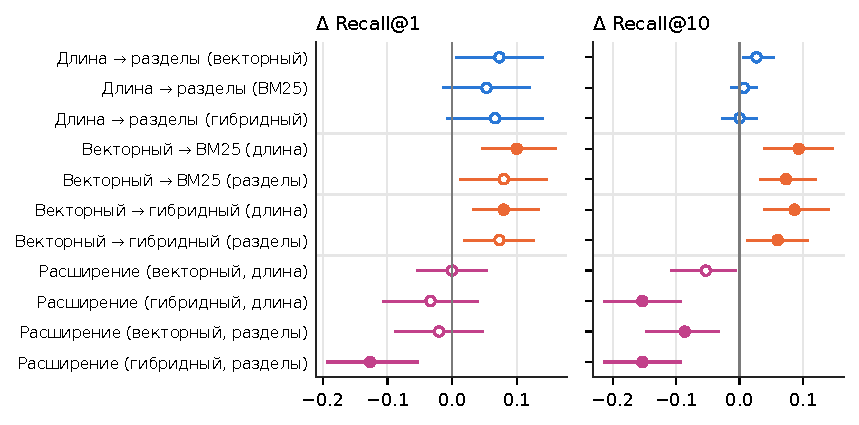
\includegraphics[width=\textwidth]{mtalk_effects}
        \end{column}
        \begin{column}{0.38\textwidth}
            \footnotesize
            {\color{soft}Берем пары прогонов, отличающиеся одним фактором, и считаем разность метрики на тех же вопросах. Отрезок показывает 95\% интервал, заполненный кружок значим с поправкой Холма.}

            \medskip
            \begin{itemize}
                \item BM25 и гибридный поиск лучше векторного, по $\Rk{10}$ значимо во всех четырех парах.
                \item Расширение снижает $\Rk{10}$ на 0,05--0,15, из топ-10 выпадает до 24 вопросов.
                \item Разделы дают +0,05--0,07 к $\Rk{1}$ в трех парах из трех, но ни одна пара не значима отдельно.
            \end{itemize}
        \end{column}
    \end{columns}
\end{frame}

%%%%%%%%%%%%%%%%%%%%%%%%%%%%%%%%%%%%%%%%%%%%%%%%%%%%%%%%%%%%
\begin{frame}{Где теряется качество}
    \footnotesize
    {\color{soft}Делим вопросы по разделу с ответом и смотрим, попали ли в топ-10 нужный патент и фрагмент с ответом.}

    \centering
    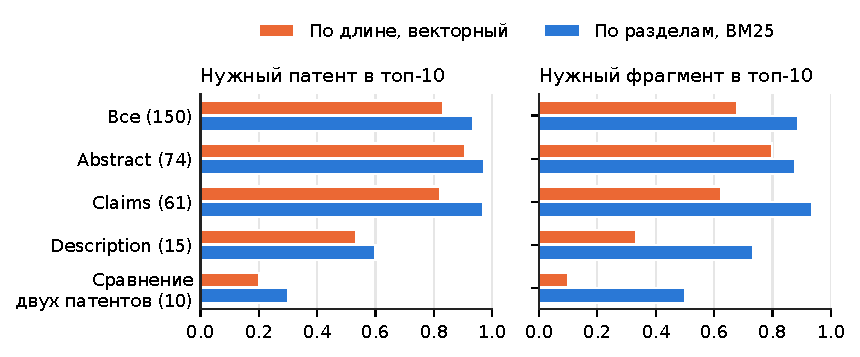
\includegraphics[width=0.72\textwidth]{mtalk_errors}

    \raggedright
    \begin{itemize}
        \item Описание: нужный абзац теряется среди десятков похожих фрагментов.
        \item Сравнения двух патентов: засчитывается один из двух, 5 из 7 вопросов не нашел ни один прогон.
        \item Переранжировщик ограничен топ-50, где нужный патент есть у 95\% вопросов с BM25 и у 85--89\% с векторным поиском.
    \end{itemize}
\end{frame}

%%%%%%%%%%%%%%%%%%%%%%%%%%%%%%%%%%%%%%%%%%%%%%%%%%%%%%%%%%%%
\begin{frame}{Где лежат ответы}
    \begin{columns}[c]
        \begin{column}{0.6\textwidth}
            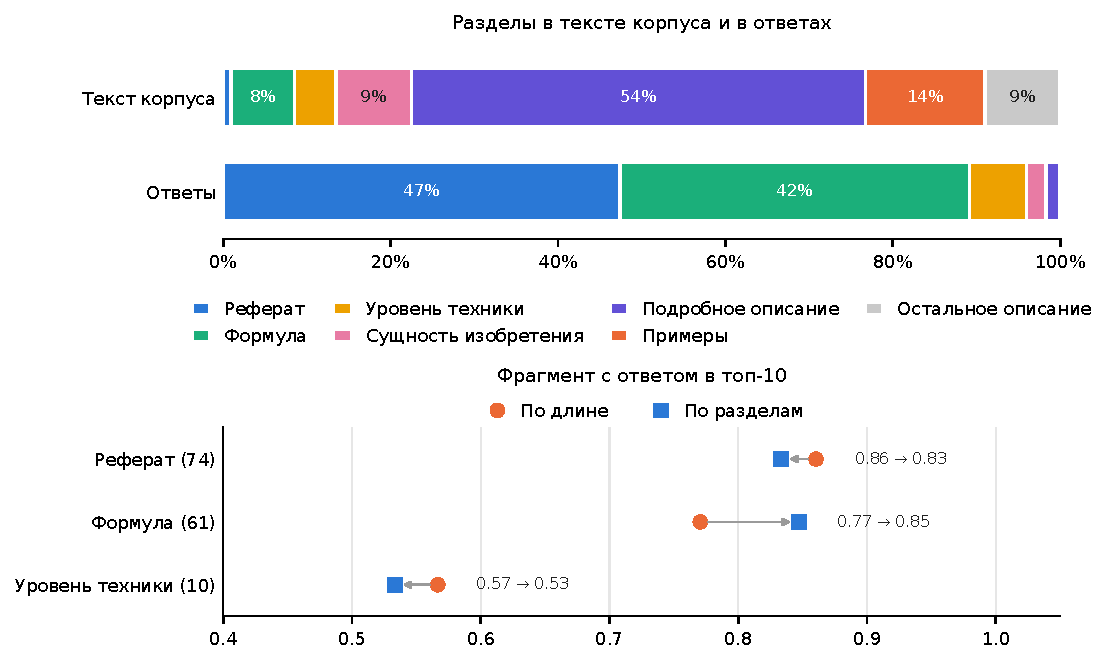
\includegraphics[width=\textwidth]{answer_sections}
        \end{column}
        \begin{column}{0.38\textwidth}
            \footnotesize
            {\color{soft}Для каждого из 175 доказательств находим раздел патента тем же кодом, что строит индекс, и сравниваем с долей текста раздела в корпусе.}

            \medskip
            \begin{itemize}
                \item 89\% ответов в реферате и формуле, хотя это 9\% текста. В реферате ответов на единицу текста в 50 раз больше среднего.
                \item Подробное описание занимает 54\% текста, но в нем всего 3 ответа, в примерах ни одного.
                \item Разбиение по разделам заметнее всего помогает формуле: 0,85 против 0,77.
                \item Вопросы по уровню техники самые трудные.
            \end{itemize}
        \end{column}
    \end{columns}
\end{frame}

%%%%%%%%%%%%%%%%%%%%%%%%%%%%%%%%%%%%%%%%%%%%%%%%%%%%%%%%%%%%
\begin{frame}{Выводы}
    \footnotesize
    \begin{columns}[T]
        \begin{column}{0.52\textwidth}
            \begin{exampleblock}{Выводы}
                \begin{enumerate}[1)]
                    \item Разделы патента находятся автоматически почти у всех патентов корпуса.
                    \item Разбиение по разделам улучшает $\Rk{1}$ после переранжирования на 0,05--0,07, но на 150 вопросах это не значимо.
                    \item Способ поиска важнее разбиения: BM25 и гибридный поиск значимо точнее векторного.
                    \item Расширение запросов языковой моделью в текущем виде вредит.
                \end{enumerate}
            \end{exampleblock}
        \end{column}
        \begin{column}{0.44\textwidth}
            \begin{alertblock}{Ограничения}
                Половина вопросов содержит термин, встречающийся не более чем в 5 патентах корпуса, и это подыгрывает BM25.
                Экспертная проверка вопросов не завершена.
            \end{alertblock}
            \begin{block}{Планы}
                \begin{itemize}
                    \item Сравнить с группировкой абзацев и RAPTOR.
                    \item Проверить окна 5 и 20 предложений.
                    \item Оценить вклад каждого раздела отдельными индексами.
                    \item Добавить вопросы по описанию.
                \end{itemize}
            \end{block}
        \end{column}
    \end{columns}
\end{frame}

\end{document}
